%************************************************
\section{Monitoring Service} % (fold)
\label{sec:impl_monitoring_service}
%************************************************
The monitoring service is meant to categorise objects in the agent's surroundings into SSM Sets. Moreover, it initializes the API \ref{sec:impl_api} and the context client \ref{sec:impl_context_client} components. Following the design we have established in Section \ref{sec:monitoring_service}, the monitoring service is implemented into several classes as depicted in Figure \ref{fig:impl_monitoring_service}.\\

The EgocentricContextManager extends the AbstractAppState class in the JME core library. On \emph{initialize()} it goes through each node in the scene graph using the WorldSpaceVisitor and adds each Spatial containing EgocentricContextData to the World Space set in the SSMBundle; more on the SSMBundle in Section \ref{subsec:impl_ssm_bundle}. The world space is computed only once, when the simulation is initialized. The WorldSpaceVisitor follows the visitor design pattern \cite{gamma1994design}.\\
\begin{figure}[H]
	\centering
	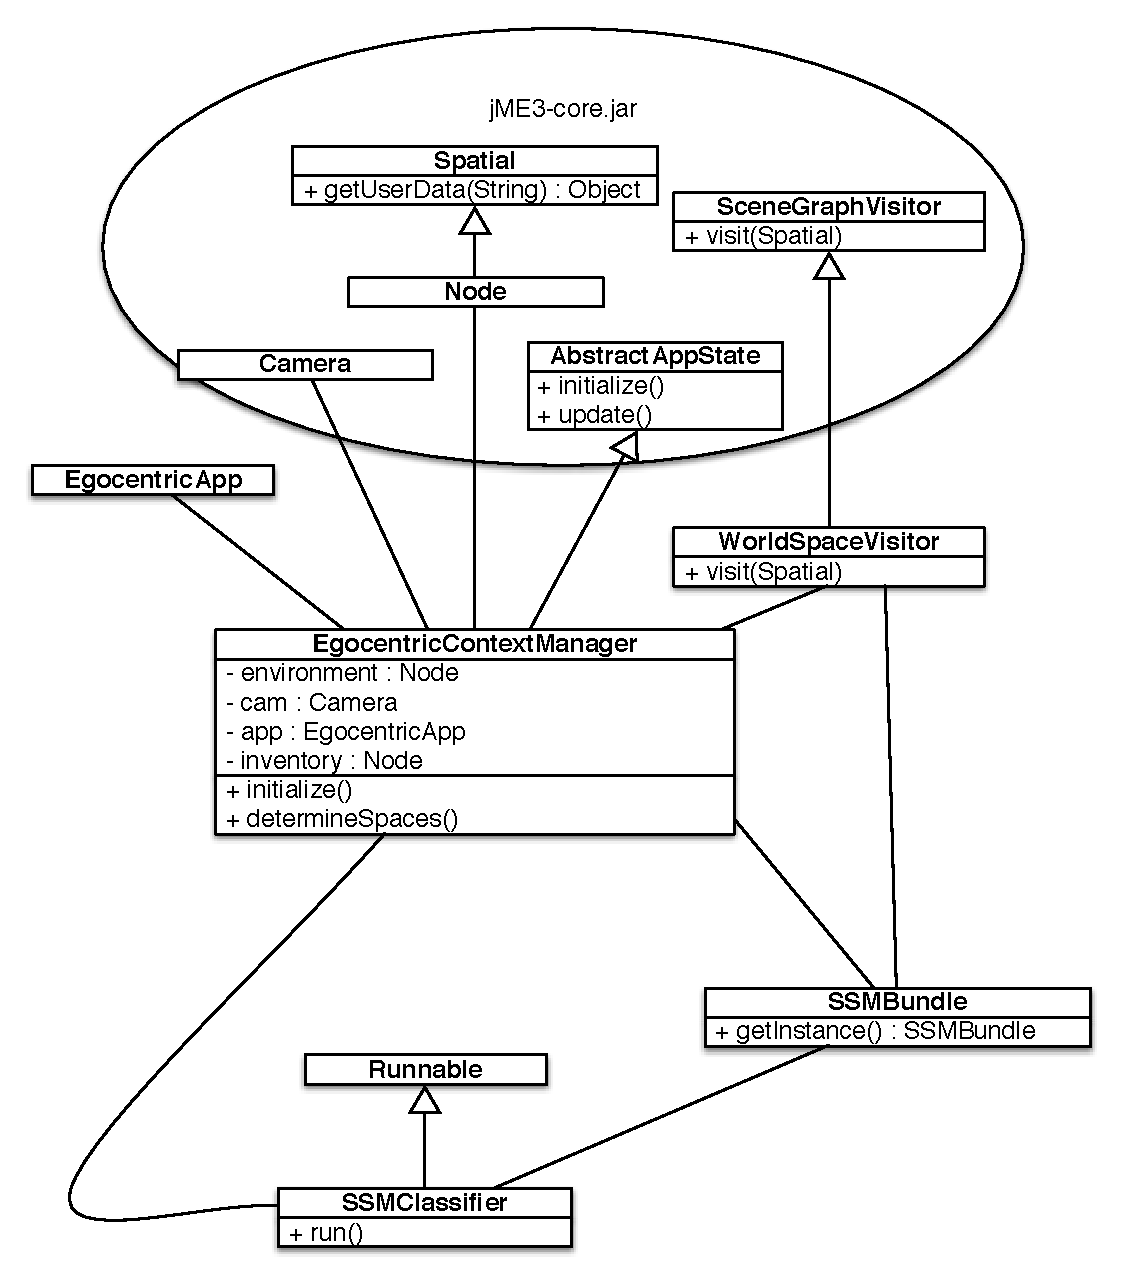
\includegraphics[width=\linewidth]{gfx/Chapter4/monitoring_service}
	\caption{Context Manager class diagram}
	\label{fig:impl_monitoring_service}
\end{figure}

The agent starts up the classification process by calling the \emph{determineSpaces()} method of the active EgocentricContextManager state instance. The classification process runs in a separate thread, the SSMClassifier.\\

%************************************************
\section{The classifier thread} % (fold)
\label{subsec:impl_the_classifier}
%************************************************
Initially, we have ran the classification within the state instance. This lead to performance issue as heavy computation was running on the UI thread, creating a disruptive user experience, sometimes heavily lagging the rendering process. Moreover, the agent triggers a new classification multiple times per second (this depends on the number of frames per second the simulation is running at) resulting in a classification being triggered before the previous one had finished. In the current implementation we allow only one classification to run at a time to avoid overlapping results. The process could be improved in the future by running multiple classifications and taking into account the results from the most recent one. However, this improvement would need thorough testing in order to avoid false positives.\\

The SSMClassifier classifies only the objects in the world space, as those are the one carrying EgocentricContextData. This approach drastically reduces the computation time as we don't have to parse the whole scene graph every time a new classification is triggered; and performance is imperative for the classification process as it needs to happen in real-time.\\

The classification logic is spread among multiple classes as depicted in Figure \ref{fig:impl_computation_strategy}. This architecture was designed to be extensible, based on the strategy design pattern \cite{gamma1994design}. Therefore, the AbstractProximitySSMSpaceComputationStrategy is a class hierarchy specialised at classifying objects in the agent's surroundings based on proximity. But the AbstractSSMSpaceComputationStrategy could be extended with other specialised hierarchies. For example, to classify objects around the agent in its audible field.
\begin{figure}[H]
	\centering
	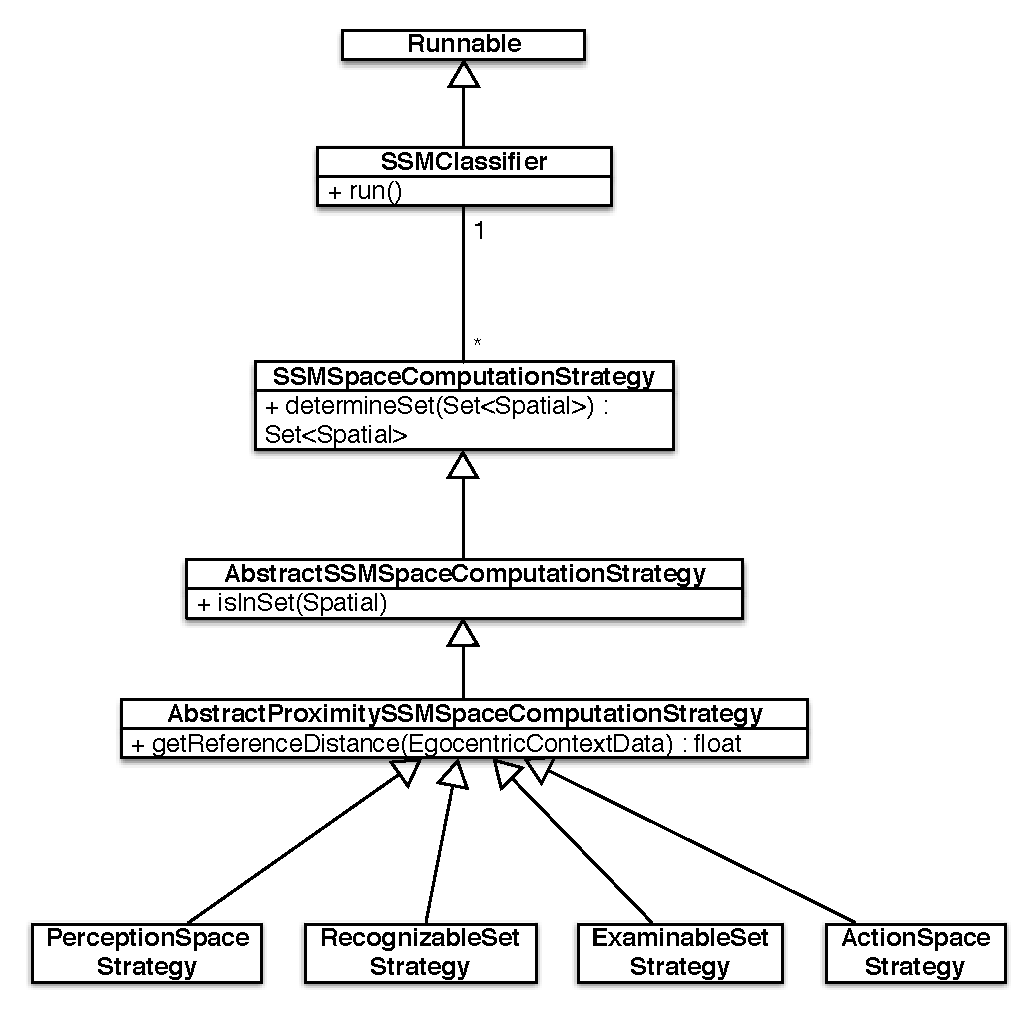
\includegraphics[width=\linewidth]{gfx/Chapter4/computation_strategy}
	\caption{Computation Strategy class diagram}
	\label{fig:impl_computation_strategy}
\end{figure}

When the classification process is started up, it first determines the set of objects in the agent's field of vision. The algorithm of determining whether an object is currently visible to the agent or not, is embedded in the SSMClassifier.isOnScreen(Spatial) method. Having the list of currently visible objects, each concrete strategy (i.e. PerceptionSpaceStrategy) is responsible to determine which of these objects should be part of a certain space.\\

After the classification process is finished, all the sets in the SSMBundle are up to date.
% section impl_the_classifier (end)

%************************************************
\section{SSM Bundle} % (fold)
\label{subsec:impl_ssm_bundle}
%************************************************
The SSMBundle is a singleton containing the SSM Sets used throughout the application. It is a shared resource and all the other components have access to it. The monitoring service updates the sets as classifications are carried out, the API and context client access the sets to provide this context information to third party clients, the agent uses the information in the sets to implement the business logic for various types of interaction.\\

Being a resource shared among multiple components and several threads, thread safety is imperative for the SSMBundle. Therefore, only one thread can access/modify the content of this resource at a time.
% section impl_ssm_bundle (end)

% section impl_monitoring_service (end)